\chapter{中央データベースとローカルデータベースのデータ同期ツールに関する研究}

開発した機能が生産時に十分であるかどうか見積もりは今後の開発を効率よく進めていく上で重要である。
生産時のデータの数や量を想定してその際のシステム性能を見積もることで、今の実装で十分かどうか、改善が必要な場合どのように改善すればいいかを知ることができる。
中央データベースとローカルデータベースのデータ同期機能に関して処理時間評価を行った。
詳細について以下で説明する。

\section{データ同期ツールに使用するAPI}
TBC

\section{サーバーの設置場所による処理時間の違い}
4章で述べたように、中央データベースはチェコに設置されている。
そのため試験結果のアップロードに関して、各組み立て機関から接続しデータ送信する処理時間は、機関の場所に大きく依存すると考えられる。
世界的にデータ同期ツールが不自由なく動くことに向けた開発、改善に役立てることを目的として、データを送信する処理時間を、以下の3つの場所に置かれているサーバーを用いて測定した。

\begin{itemize}
  \item 日本、高エネルギー加速器研究所(KEK) 
  \item アメリカ、バークレー研究所(LBL)
  \item スイス、欧州原子核研究機構(CERN)
\end{itemize}

各サーバーの性能を表\ref{server_spec}に示す。また各サーバーが置かれている場所の位置関係を図\ref{server_position}に示す。

\begin{table}[tbp]
\caption[サーバーの性能一覧]{サーバーの性能一覧}
\label{server_spec}
\scalebox{0.9}{
  \begin{tabular}{|l|llll|l|l|} \hline
    設置機関 & CPU & & & & Memory & Disk \\
     & Type & Core & Thread & Clock speed[GHz]& [kB] & [GB] \\ \hline 
    KEK & Intel(R) Core(TM) i7-6700 & 4 & 8 & 3.4 & 15,981,000 & 197\\
    LBL & Intel(R) Core(TM) i7-8700 & 6 & 12 & 3.7 & 32,628,000 & 233\\
    CERN & Intel Core Processor (Broadwell, IBRS) & 1 & 10 & 2.2 & 29,978,888 & 80\\ \hline
  \end{tabular}
}
\end{table}


\begin{figure}[bpt]\centering

\includegraphics[width=1cm]{figure}
\caption[各サーバの位置関係]{各サーバの位置関係}
\label{server_position}
\end{figure}

これらのサーバーは実際に生産の際に使用するものと同程度の性能を持ち、サーバーが置かれている環境も生産時と同じであるとしている。
回線の混雑具合などによる処理時間の低下は、本測定では考慮に入れていない。

\subsection{登録モジュール情報の取得にかかる時間}
ある登録されたモジュール情報の取得にかかる時間を測定した。
各サーバーでの処理時間についてまとめたものを表\ref{getting_1module}に示す。

\begin{table}[tbp]
\begin{center}
\caption[モジュール情報の取得にかかる時間]{モジュール情報の取得にかかる時間}
\label{getting_1module}
  \begin{tabular}{|ll|} \hline
    サーバー & 処理時間 \\ \hline
    KEK & 0.49 $\pm$ 0.02 \\ 
    LBL & 0.37 $\pm$ 0.02 \\ 
    CERN & 0.30 $\pm$ 0.04 \\ \hline 
  \end{tabular}
\end{center}
\end{table}

\subsection{1Byteのデータファイル送信にかかる時間}
ある試験結果ページに、Attachmentとして1Byteのデータファイルを送信する時間を測定した。
各サーバーでの処理時間についてまとめたものを表\ref{sendpd_1byte}に示す。

\begin{table}[tbp]
\begin{center}
\caption[1Byteのデータファイル送信にかかる処理時間]{1Byteのデータファイル送信にかかる処理時間}
\label{sendpd_1byte}
  \begin{tabular}{|ll|} \hline
    サーバー & 処理時間 \\ \hline
    KEK & 0.54 $\pm$ 0.04 \\ 
    LBL & 0.34 $\pm$ 0.03 \\ 
    CERN & 0.39 $\pm$ 0.02 \\ \hline 
  \end{tabular}
\end{center}
\end{table}

\subsection{データファイル送信処理時間の容量依存性}
ある試験結果ページに、Attachmentとしてデータファイルを送信する時間をいくつかのファイルサイズにおいて測定した。
ファイルサイズと処理時間の関係を図\ref{datasize_vs_time}に示す。上述した1Byteでの測定点も含んでいる。

\begin{figure}[bpt]\centering
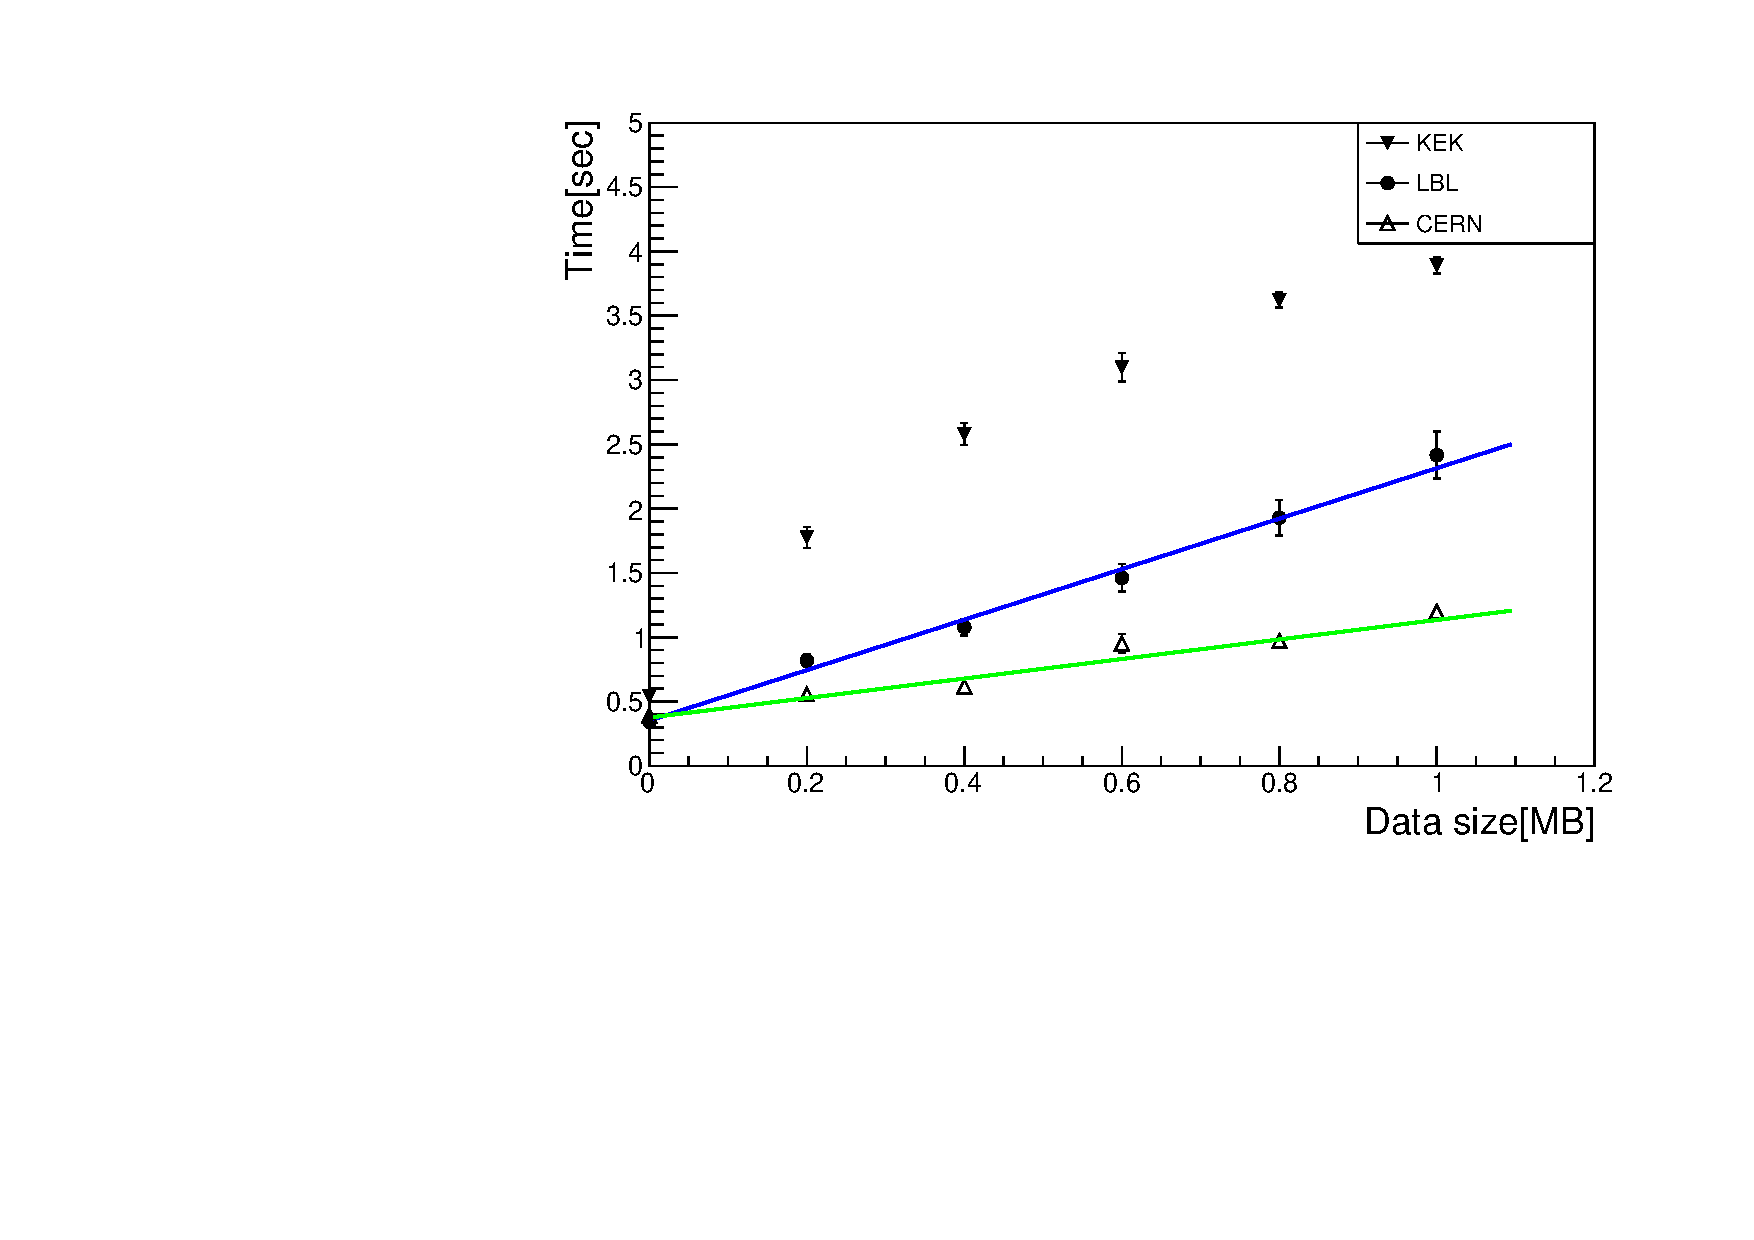
\includegraphics[width=9cm,angle=270]{datasize_vs_time.pdf}
\caption[送信するファイルサイズと処理時間の関係]{送信するファイルサイズと処理時間の関係}
\label{datasize_vs_time}
\end{figure}

\section{モジュールIDのダウンロード機能確認と処理時間測定}
\subsection{アルゴリズム}
\subsection{機能確認}
KEKのモジュール登録とダウンロード機能の確認。
\subsection{処理時間測定}
工夫点
\section{読み出し試験結果のアップロード機能確認と処理時間測定}
\subsection{アルゴリズム}
\subsection{機能確認}
\subsection{処理時間測定}

工夫点

